\section{Model Checking}
\subsection{Introduction}
To build our final model, we decided to use an incremental way of construction, meaning that we started from a Minimum Viable Product that we develop more a little bit more at each step. We did verify each one and that way we are sure we have a correct base and can identify issue more easily.

At the end of the day, we did it in 4 different steps. We will now, without entering in the details for the first steps, explain what can be done there. The final step will be deeply explained since it is the most complex one.

\subsubsection{Step 1: Basic Traffic Lights system}
In this first basic step, we created the model in Uppaal of a simple controller sending a pulse every 3 seconds to two cars traffic lights. There is no pedestrians and no buses in this step. \\
Every 3 seconds, the South and North traffic lights switch from green to red while the East and West traffic lights switch, on the opposite, from red to green. \\

Thanks to this basic example, we understood Uppaal basics and notably how it is possible to send messages from one component to an other component thanks to the channel message passing system. \\

In this system, it is possible to check whether our first traffic light is green and the other is red at certain time and vice-versa. Thus we check if we never reach a state where our system is in an impossible and dangerous state where both traffic lights would be green.


\begin{figure}[!ht]\label{fig:arduino}
  \centering
    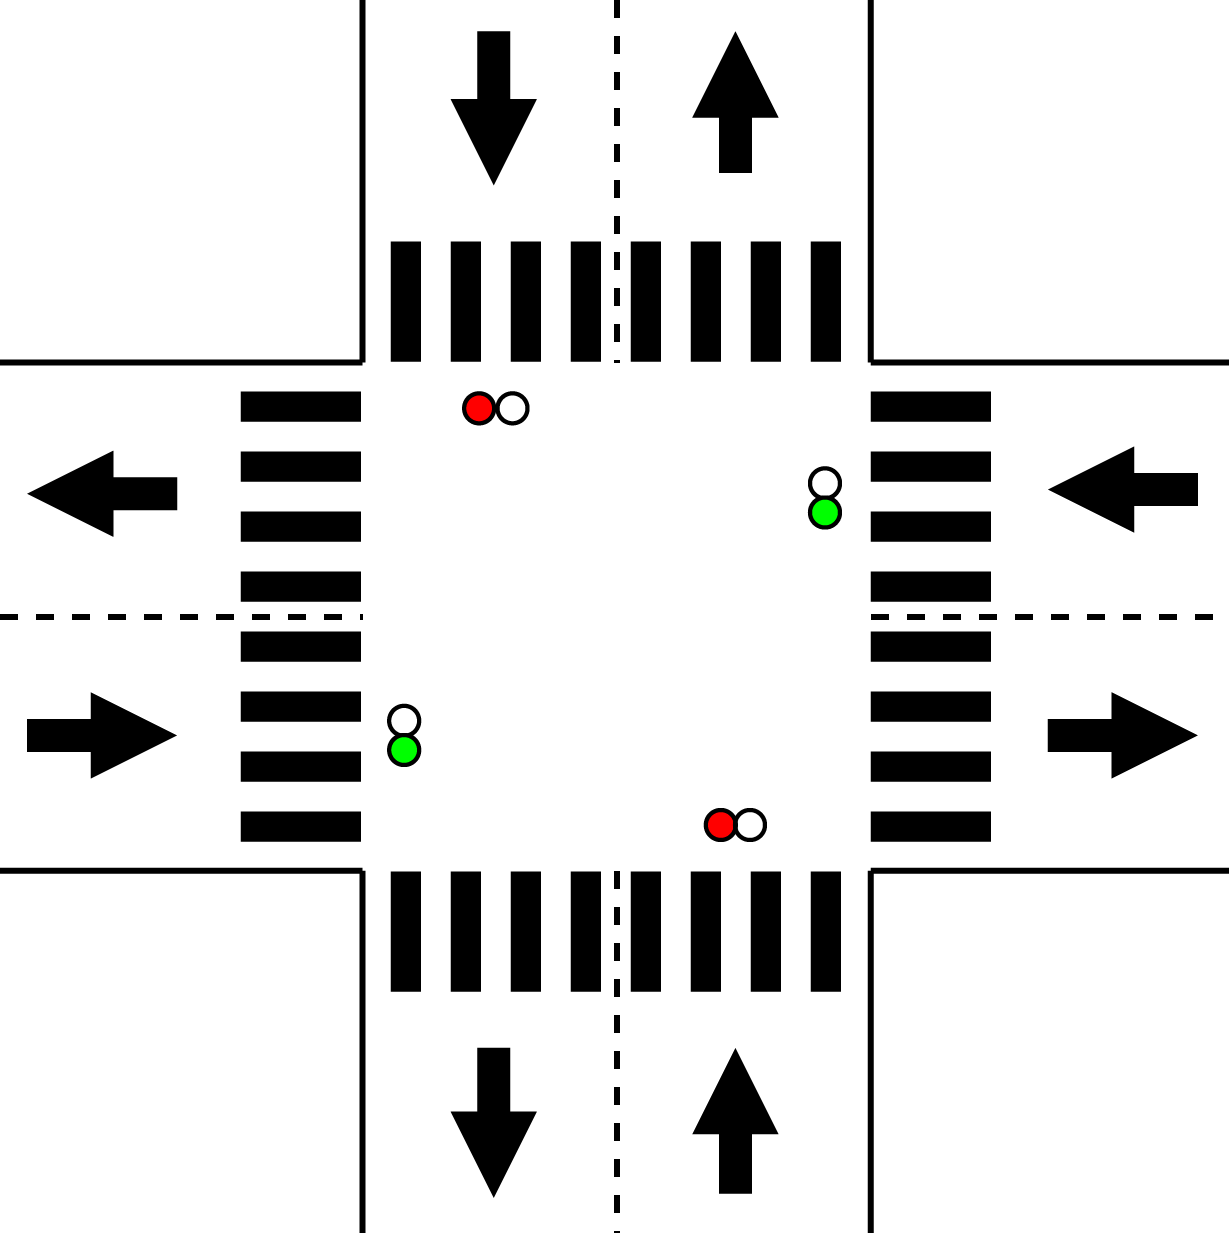
\includegraphics[width=0.5\textwidth]{picture/model/trafficlight_step1_s1.png}
    \caption{Arduino Due used for the embedded system}
\end{figure}

\subsubsection{Step 2: Pedestrians}
In this step, pedestrians were now added and many different things had to be changed to allow accommodate this new change. \\ 

When a pedestrians call was send by the environment, the car's traffic light that was green had to become red and the other car traffic light had to stay red. When those two traffic lights are red, the pedestrians traffic light could be green. Because we also wanted fairness in our system, two assumptions were here created.
\begin{enumerate}
    \item When the pedestrians traffic light is green, we have to remember which car traffic light was previously green. This will be useful for the next assumption.
    \item We wanted fairness between the actors, even if pedestrians have the priority. The problem at the beginning was that starvation could happen if, when the pedestrians lights are green, we always switched to a specific car's traffic light. This would mean that the other car's traffic light would remain red if pedestrians are always calling. We thus added what we called a "delayed" call where, even if the pedestrians are always pressing the button, the two cars lights have to be green at least once before the pedestrians could have their lights green again. This is why the first assumption is useful, we have to remember which car's light was previously green so the cars in the other side of the crossroad don't always have to wait 2 times to be green again. \\
    As an example, if the East-West car's traffic light is green and a pedestrian pressed the button, after the pedestrians lights switch from green to red, the North-South car's traffic light is switched to green so they do not have to wait another time.
\end{enumerate}
In this step, more properties were checked. We for example check if, after a transition, the value of a component always reaches the enquired value. We also check, as for the first one, that certain states can never be reached in our model (all traffic lights are green for example).

\begin{figure}[!ht]\label{fig:arduino}
  \centering
    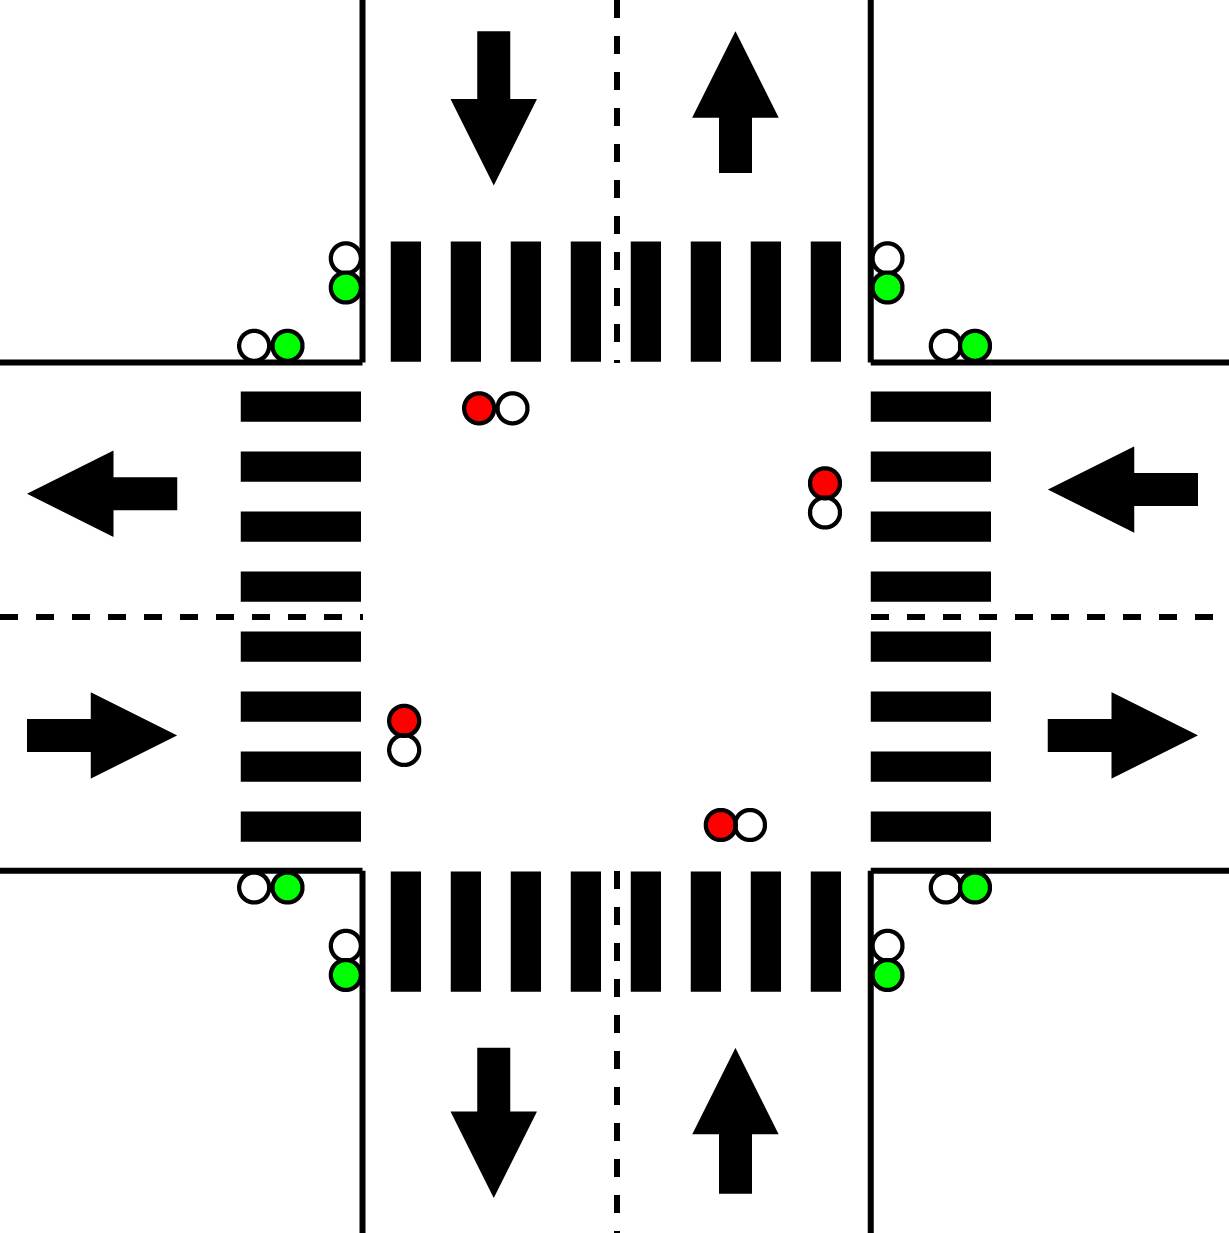
\includegraphics[width=0.5\textwidth]{picture/model/trafficlight_step2_s3.png}
    \caption{Arduino Due used for the embedded system}
\end{figure}

\subsubsection{Step 3: Buses}
In this step, we added the buses generated by the environment. The idea here is that the buses have priority on the rest of the traffic. \\
When a bus is generated, the next traffic light that has to be green is the one of the bus. When the bus is crossing, all other lights are red because the bus will go through all the crossroad. \\
Even if the pedestrians have called to have the green lights before the bus, if a bus is generated between the call and the pedestrians green light, we will first give the green light for the bus, then the pedestrians, then the cars. This mean that the priority hierarchy is \textit{Buses-Pedestrians-Cars}. 


\begin{figure}[!ht]\label{fig:arduino}
  \centering
    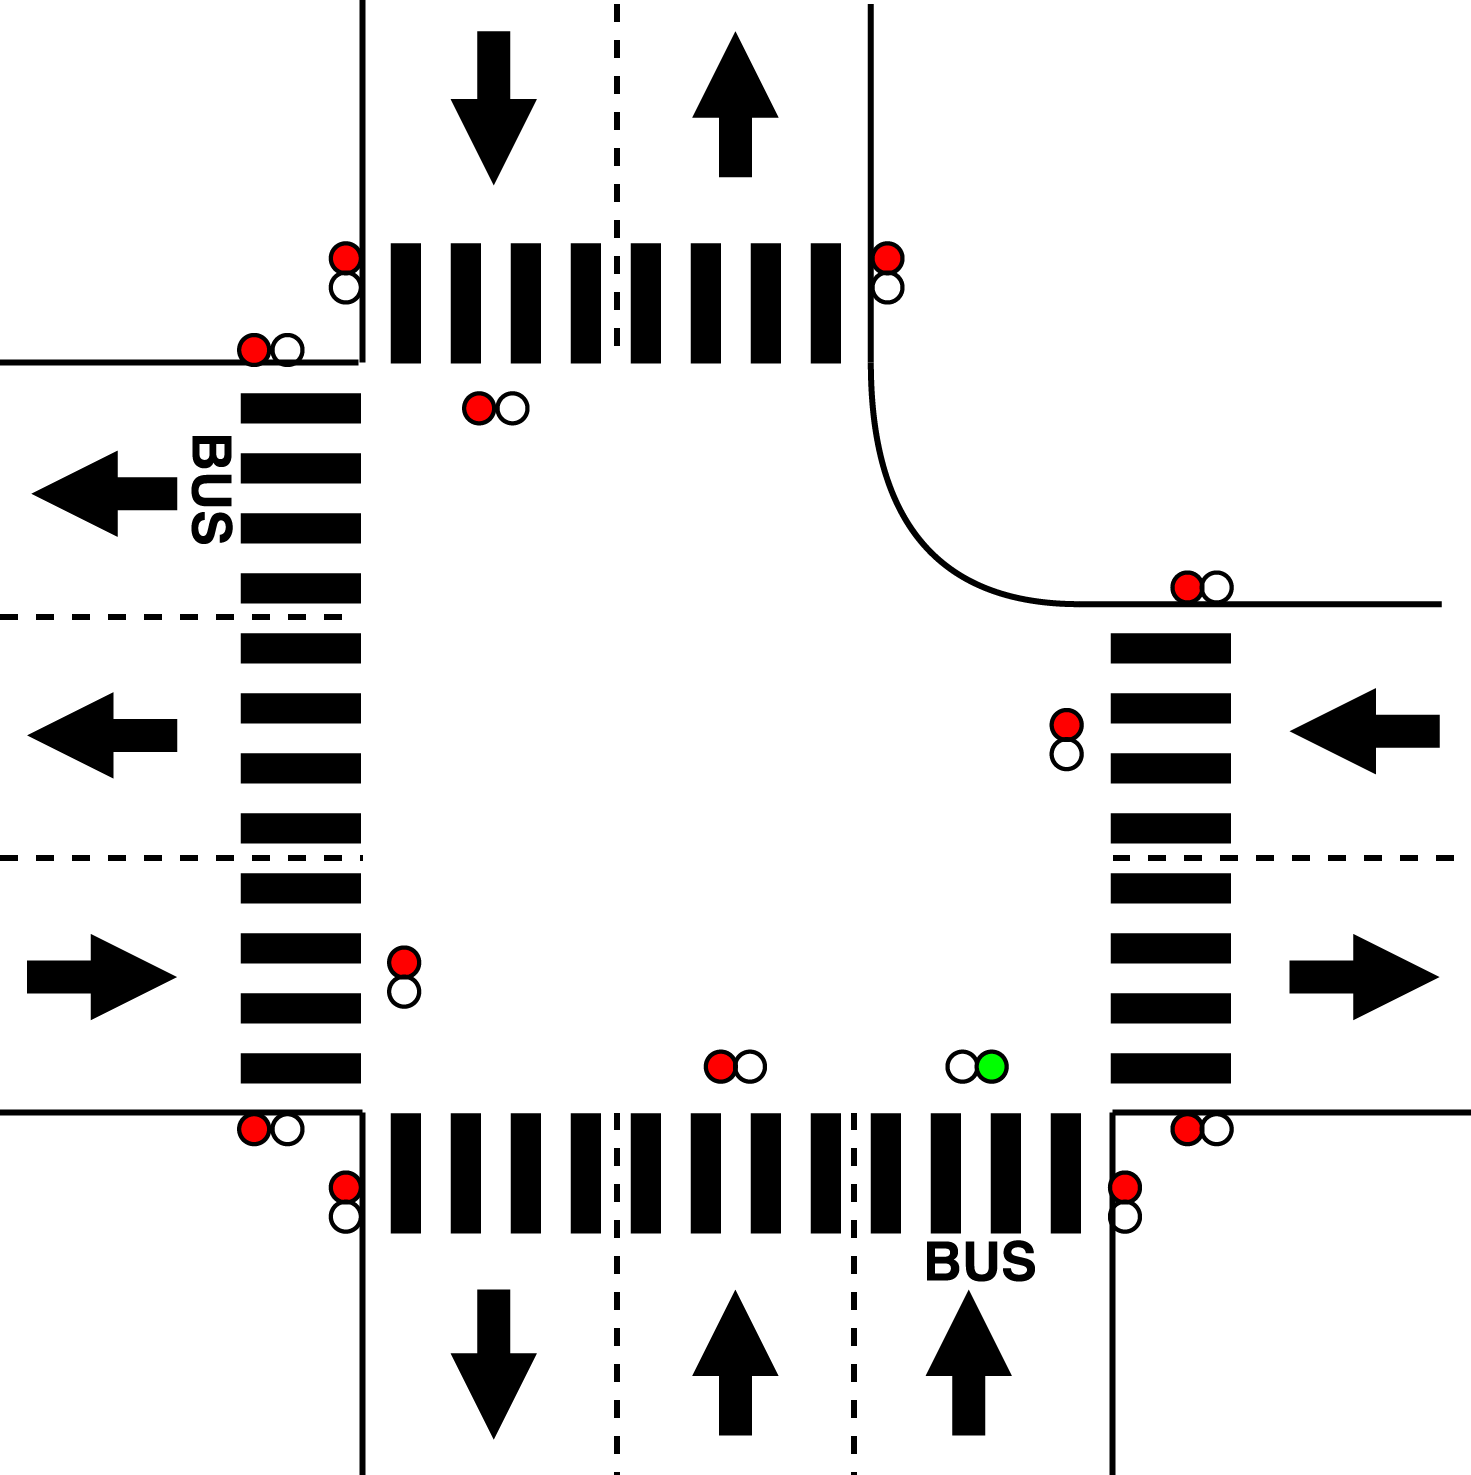
\includegraphics[width=0.5\textwidth]{picture/model/trafficlight_step3_s2.png}
    \caption{Arduino Due used for the embedded system}
\end{figure}

\subsubsection{Step 4: Yellow Light}
For this step, we kept the same model done in step 3 but we added a yellow light. This means that, as in the real life, our cars traffic lights will switch from green to yellow to red. \\
This is thus our final model developed in Uppaal TiGa.

\begin{figure}[!ht]\label{fig:arduino}
  \centering
    \includegraphics[width=0.5\textwidth]{picture/model/Trafficlight_step4.png}
    \caption{Arduino Due used for the embedded system}
\end{figure}

\subsection{Timed Automatons}
In order to formally model the system, we use several timed automatons from Uppaal. While some of those automatons are actors in the environment, the others are part of the controller.
The theory tells us that, when the environment is playing, we, humans, cannot decide the action that will be taken. For example, buses and pedestrians arrivals are unpredictable and uncontrollable, so they belong to the environment.
The actors which implement the solution for avoiding crashes belong to the controller. They interact with the environment in order to avoid crashes and thus they aim to find a winning strategy.
